\documentclass[svgnames, 12pt]{beamer}

%----------------------------------------------------------------------------------------
%   PACKAGES AND THEMES
%----------------------------------------------------------------------------------------

\usepackage[utf8]{inputenc}
\usepackage[english]{babel}
\usepackage[L7x]{fontenc}
\usepackage{lmodern}
\usepackage{amsmath}
\usepackage{amssymb}
\usepackage{xcolor}
\usepackage{subfig}
\usepackage{graphicx}
\usepackage{lipsum}
\usepackage{hyperref}
\usepackage{booktabs}

\definecolor{mifcolor}{RGB}{0, 71, 127}
\definecolor{dimgr}{RGB}{105, 105, 105}
\definecolor{sky}{RGB}{0, 191, 255}
\setbeamercolor{alerted text}{fg=red,bg=sky}
\newcommand{\boxalert}[1]{{
	\usebeamercolor{alerted text}\colorbox{bg}{\alert{#1}}
}}

\mode<presentation>{
	\usetheme{Madrid}
	\usecolortheme[named=mifcolor]{structure}
	\setbeamertemplate{footline}
	{
		\leavevmode
		\hbox{
			\begin{beamercolorbox}[wd=.3\paperwidth,ht=2.5ex,dp=1.125ex,leftskip=.3cm
				plus1fill,rightskip=.3cm]{author in head/foot}
				\usebeamerfont{author in head/foot}\insertshortauthor \hfill
			\end{beamercolorbox}
			\begin{beamercolorbox}[wd=.2\paperwidth,ht=2.5ex,dp=1.125ex,leftskip=.3cm,
				rightskip=.3cm plus1fil]{institute in head/foot}
				\usebeamerfont{institute in head/foot}\insertshortinstitute
			\end{beamercolorbox}
			\begin{beamercolorbox}[wd=.2\paperwidth,ht=2.5ex,dp=1.125ex,leftskip=.3cm,
				rightskip=.3cm plus1fil]{date in head/foot}
				\usebeamerfont{date in head/foot}\insertshortdate
			\end{beamercolorbox}
			\begin{beamercolorbox}[wd=.3\paperwidth,ht=2.5ex,dp=1.125ex,leftskip=.3cm,
				rightskip=.3cm plus1fil]{title in head/foot}
				\usebeamerfont{title in head/foot}\insertshorttitle\hfill p.
				\insertframenumber\enspace of \inserttotalframenumber\enspace
			\end{beamercolorbox}
		}
		\vskip0pt
	}
}

\title[Air Quality Analysis in Delhi]{Multivariate Time Series Analysis of Air Quality Data in Delhi}
\author[A. J. Smoliakov]{Aleksandr Jan Smoliakov\inst{1}}
\institute[VU MIF]{\inst{1} Vilnius University, Faculty of Mathematics and Informatics}
\date{2025--05--27}

%----------------------------------------------------------------------------------------
%   BEGIN DOCUMENT
%----------------------------------------------------------------------------------------
\begin{document}

%----------------------------------------------------------------------------------------
%   TITLE FRAME
%----------------------------------------------------------------------------------------
\begin{frame}
	
\includegraphics[scale=0.15]{MIF Garamond-logo.png} 
	\hfill
	
\includegraphics[scale=0.15]{Logo_spalvotas.eps}
	\titlepage{}
\end{frame}

%----------------------------------------------------------------------------------------
%   TABLE OF CONTENTS
%----------------------------------------------------------------------------------------
\begin{frame}{Table of Contents}
\tableofcontents
\end{frame}

%----------------------------------------------------------------------------------------
\section{Introduction}
%----------------------------------------------------------------------------------------
\begin{frame}
    \frametitle{Introduction: The Air Quality Challenge}
    \begin{itemize}
        \item Urban air quality is a critical public health and environmental issue, especially in rapidly urbanizing regions like Delhi.
        \item Accurate forecasting of pollutants (e.g. $PM_{2.5}$, $PM_{10}$, $NO_2$, CO) is essential for timely policy interventions.
        \item Univariate models (e.g. ARIMA) may not capture complex interdependencies.
        \item Multivariate time series models (e.g. VAR, VARMA) can model interactions between multiple pollutant series.
    \end{itemize}
    \vspace{0.5cm}
    \begin{block}{Focus of this Project}
        Analyze air quality in Delhi (2018--2019) using daily data for five key pollutants: $PM_{2.5}$, $PM_{10}$, $NO_2$, CO, and $NH_3$.
    \end{block}
\end{frame}

%----------------------------------------------------------------------------------------
\begin{frame}
    \frametitle{Project Objectives}
    \begin{itemize}
        \item Apply multivariate time series models (VAR and VARMA) to understand the dynamic interactions among five air pollutants in Delhi.
        \item Generate forecasts for these pollutant concentrations.
        \item Key steps involved:
        \begin{itemize}
            \item Data preprocessing and Exploratory Data Analysis (EDA).
            \item Stationarity testing.
            \item VAR and VARMA model estimation.
            \item Granger causality analysis.
            \item Impulse Response Function (IRF) analysis.
            \item Forecast Error Variance Decomposition (FEVD).
            \item Forecast evaluation.
        \end{itemize}
    \end{itemize}
\end{frame}

%----------------------------------------------------------------------------------------
\section{Methodology}
%----------------------------------------------------------------------------------------
\begin{frame}
    \frametitle{Data Source and Preparation}
    \begin{itemize}
        \item \textbf{Dataset:} \textit{Air Quality Data in India (2015--2020)}.
        \item \textbf{Focus:} Delhi, Jan 1, 2018 -- Jan 1, 2020 (732 daily observations).
        \item \textbf{Pollutants:} $PM_{2.5}$, $PM_{10}$, $NO_2$, CO, $NH_3$.
        \item \textbf{Reasons for Delhi focus:}
            \begin{itemize}
                \item One of the world's most polluted cities.
                \item Relatively complete data ($<1\%$ missing values for the selected period).
            \end{itemize}
        \item \textbf{Missing Value Imputation:} Linear interpolation (\texttt{na.interp}).
        \item \textbf{Data Transformation:} $\log(x+1)$ (log1p) to stabilize variance and normalize distributions.
        \item \textbf{Data Aggregation:} Hourly data aggregated to daily means (of log1p-transformed values) to reduce noise.
    \end{itemize}
\end{frame}

%----------------------------------------------------------------------------------------
\begin{frame}
    \frametitle{Exploratory Data Analysis (EDA)}
    \begin{itemize}
        \item \textbf{Distributions after transformation:}
    \end{itemize}
    \begin{figure}
        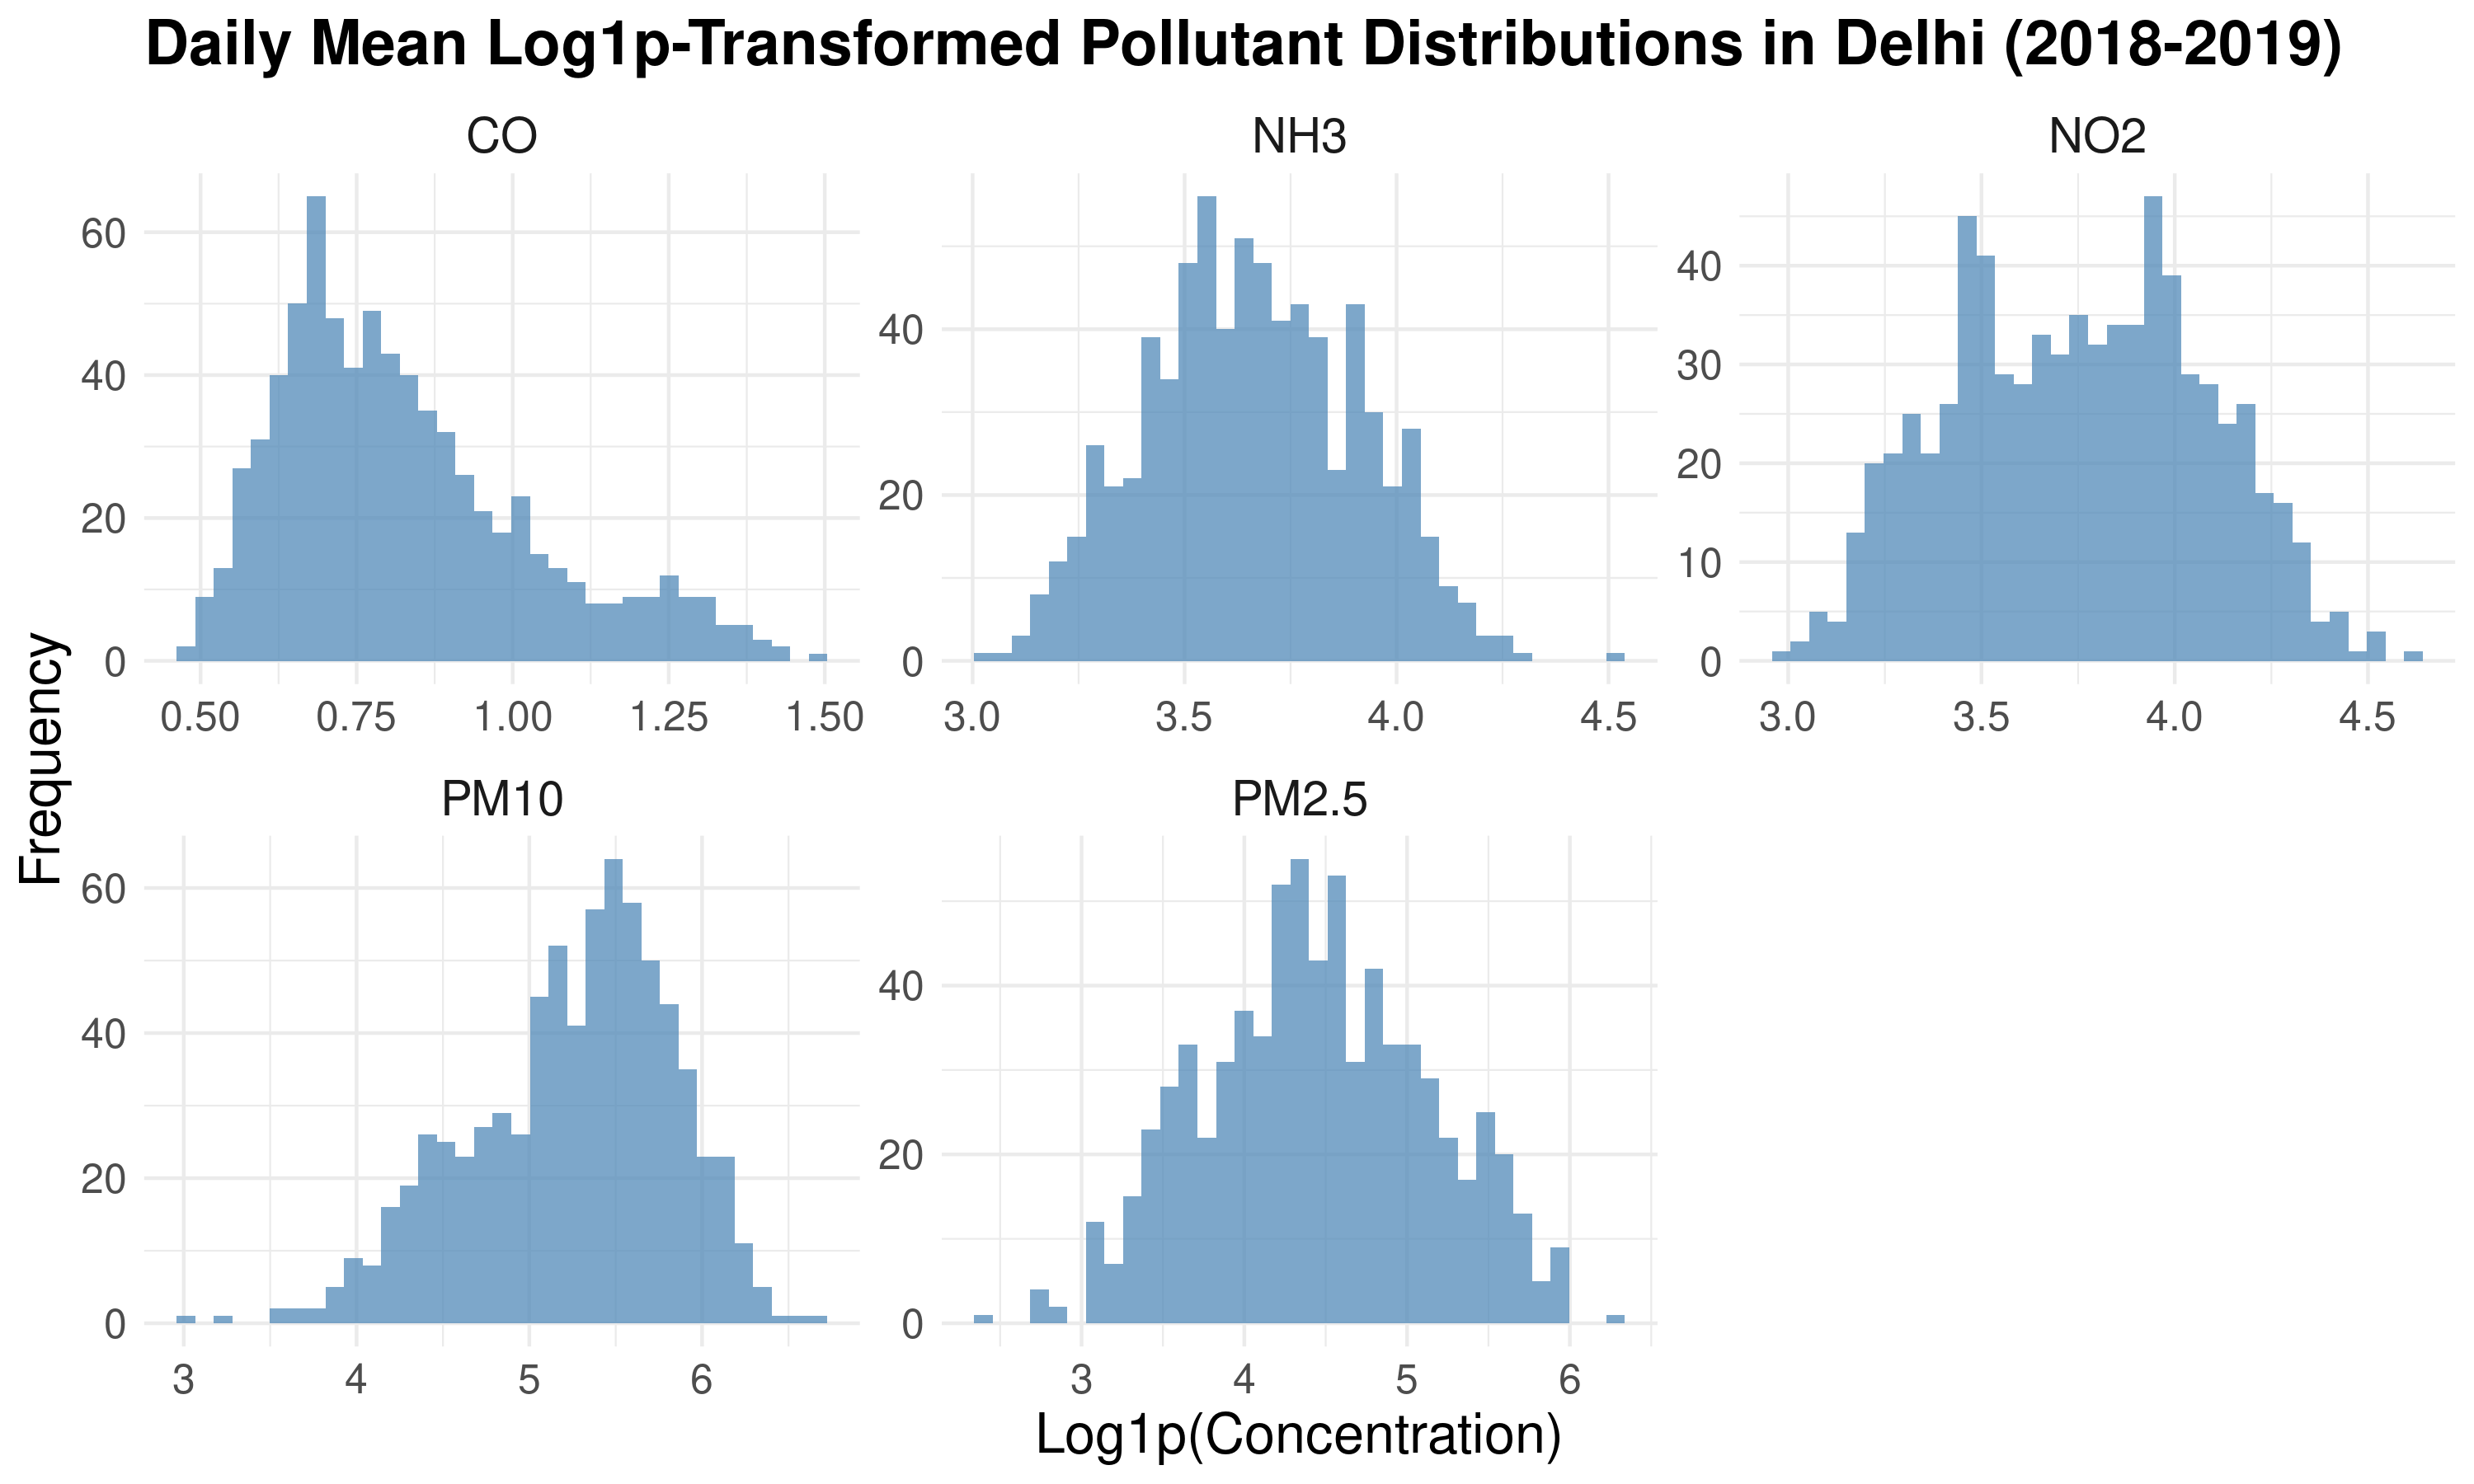
\includegraphics[width=0.8\linewidth]{../analysis/assets/log1p_delhi_distributions.png}
        \caption{Histograms of Daily Mean log1p-Transformed Pollutants (Delhi, 2018--2019).}
    \end{figure}
    \begin{itemize}
        \item Time series plots showed seasonality (higher pollution in winter).
        \item Correlation matrix revealed strong positive correlations (e.g. $PM_{2.5}$ \& $PM_{10}$: 0.93; $NO_2$ \& CO: 0.86).
    \end{itemize}
\end{frame}

%----------------------------------------------------------------------------------------
\begin{frame}
    \frametitle{EDA: Time Series and Correlations}
    \begin{columns}[T] % Split slide into two columns
        \begin{column}{0.5\textwidth}
            \textbf{Time Series Behavior:}
            \begin{figure}
                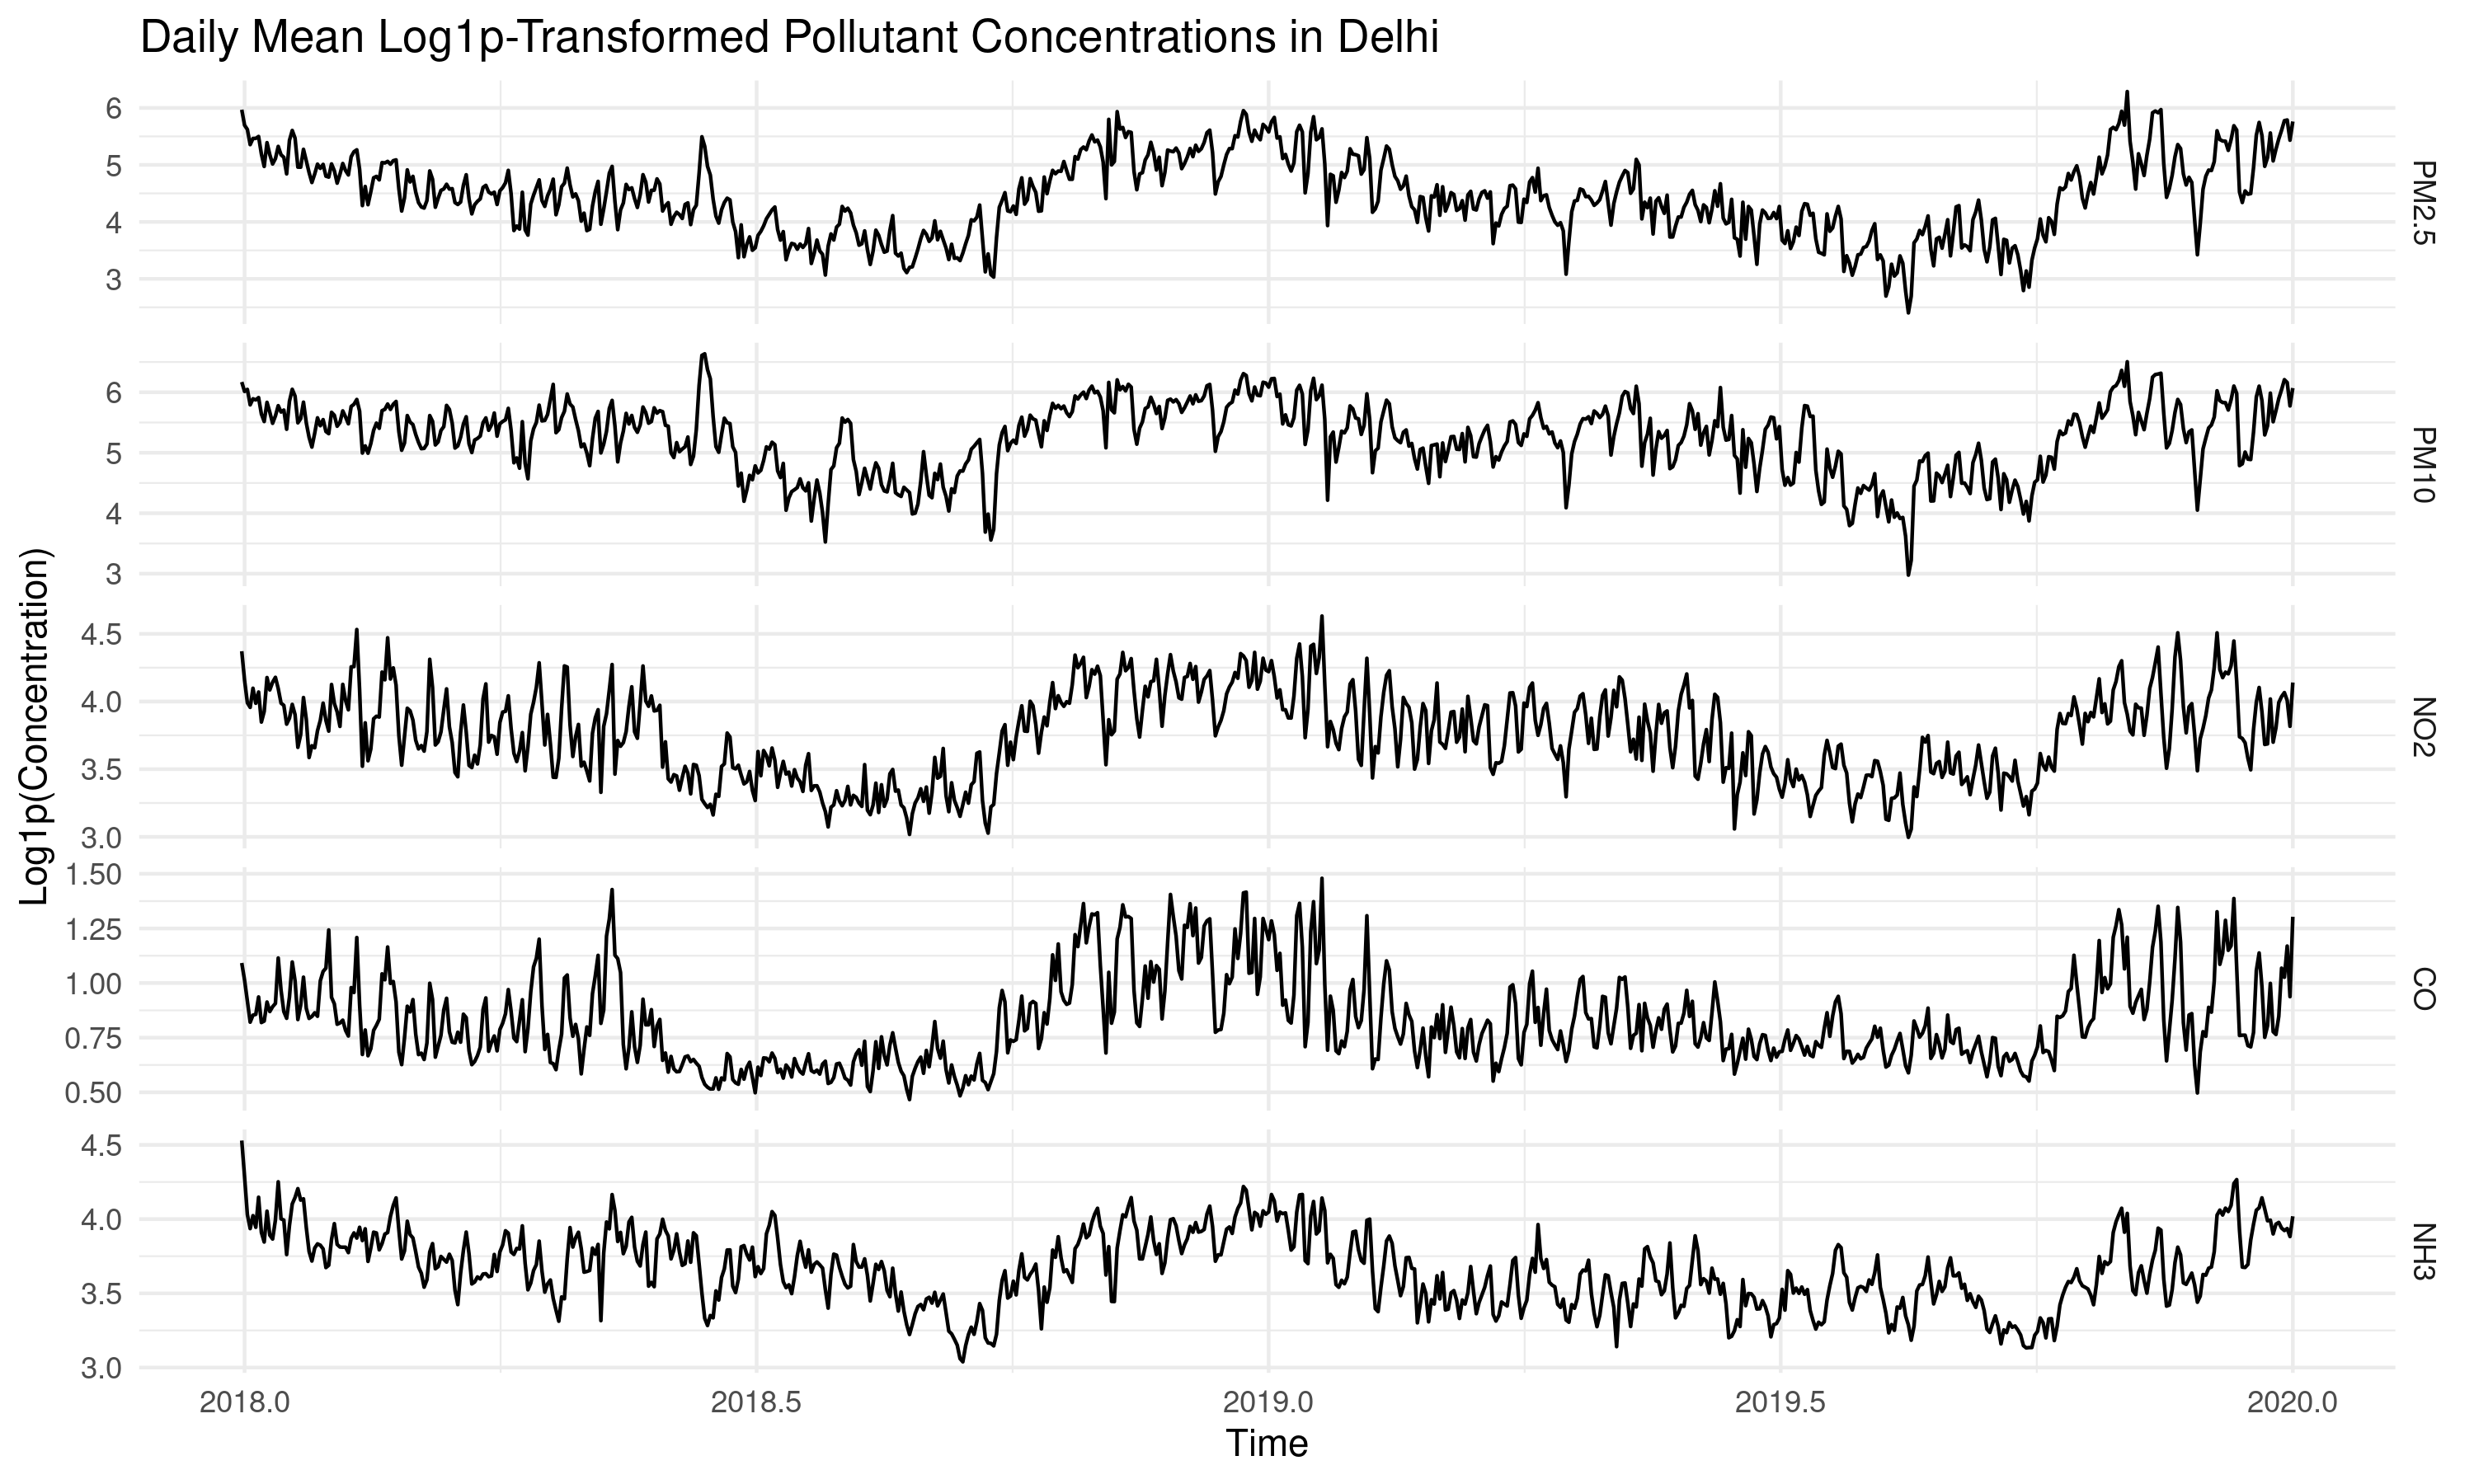
\includegraphics[width=\linewidth]{../analysis/assets/daily_ts_delhi.png}
                \caption*{Daily Log1p-Transformed Pollutants.}
            \end{figure}
        \end{column}
        \begin{column}{0.5\textwidth}
            \textbf{Correlation Matrix:}
            \begin{figure}
                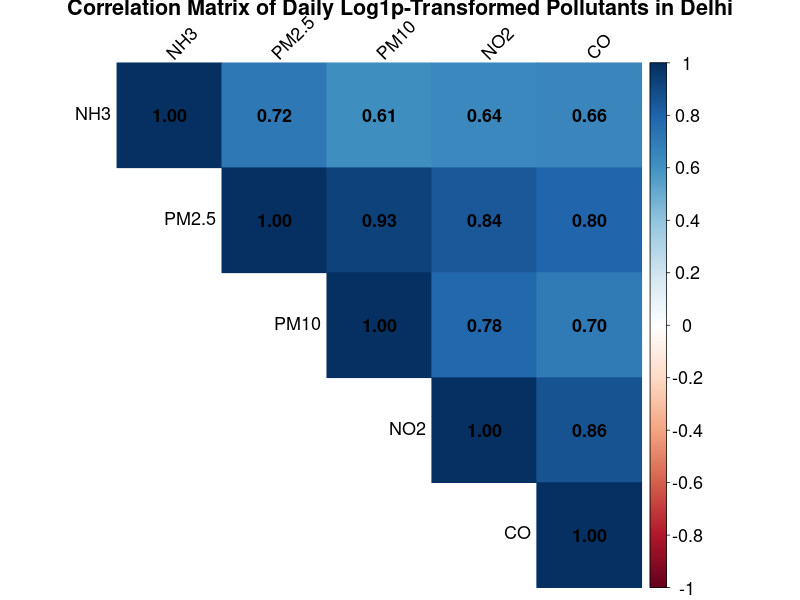
\includegraphics[width=0.9\linewidth]{../analysis/assets/corrplot_delhi.png}
                \caption*{Correlations (Log1p-Transformed).}
            \end{figure}
        \end{column}
    \end{columns}
    \footnotesize Note: Strong correlations are evident, there may be multivariate dependencies.
\end{frame}

%----------------------------------------------------------------------------------------
\begin{frame}
    \frametitle{Stationarity Testing \& Model Choices}
    \begin{itemize}
        \item \textbf{Stationarity Testing:} Augmented Dickey-Fuller (ADF) test on log1p-transformed daily series.

        Conclusion: all log1p-transformed series are stationary (I(0)) with $p < 0.01$, allowing for VAR/VARMA modeling.

        \item \textbf{Vector Autoregression (VAR) Model:}
            \[ Y_t = c + A_1 Y_{t-1} + \cdots + A_p Y_{t-p} + \epsilon_t \]
            Optimal lag $p$ via AIC (\texttt{vars::VARselect}).

        \item \textbf{Vector Autoregressive Moving Average (VARMA) Model:}
            \[ Y_t = A_1 Y_{t-1} + \cdots + A_p Y_{t-p} + B_1 \epsilon_{t-1} + \cdots + B_q \epsilon_{t-q} + \epsilon_t \]
            Only VARMA(1,1) explored, larger orders did not converge.
    \end{itemize}
\end{frame}

%----------------------------------------------------------------------------------------
\section{Results and Discussion}
%----------------------------------------------------------------------------------------
\begin{frame}
    \frametitle{VAR(4) Model Analysis: Lag Selection \& Causality}
    \begin{itemize}
        \item \textbf{Lag Order Selection for VAR:}
            \begin{itemize}
                \item VAR(4) model selected as suggested by AIC.
                \item Model stable (all roots of characteristic polynomial $<1$).
            \end{itemize}
        \item \textbf{Granger Causality (from VAR(4) model):}
            \begin{center}
            \footnotesize
            \begin{tabular}{lc}
                \toprule
                Causality Direction & $p$-value \\
                \midrule
                $PM_{2.5} \rightarrow$ Others & $4.80 \times 10^{-5}$ *** \\
                $PM_{10} \rightarrow$ Others & $9.81 \times 10^{-4}$ *** \\
                $NO_{2} \rightarrow$ Others & $0.0327$ * \\
                CO $\rightarrow$ Others & $0.174$ \\
                $NH_{3} \rightarrow$ Others & $8.56 \times 10^{-7}$ *** \\
                \bottomrule
            \end{tabular}
            \end{center}
            \vspace{0.2cm}
            \textbf{Observation:} Significant predictive relationships, especially from $PM_{2.5}$ and $NH_3$.
    \end{itemize}
\end{frame}

%----------------------------------------------------------------------------------------
\begin{frame}
    \frametitle{VAR(4) Analysis: Impulse Response Functions}
    \begin{itemize}
        \item IRFs trace the effect of a one-standard-deviation shock in one variable on others.
        \item Shown below: Response of $NO_2$ to a shock in $NH_3$.
    \end{itemize}
    \begin{figure}
        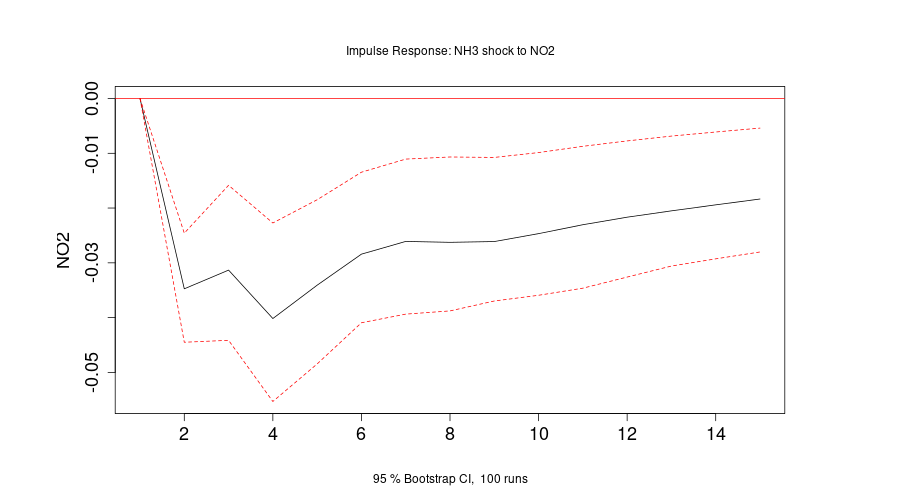
\includegraphics[width=0.9\linewidth]{../analysis/assets/irf_nh3_no2.png}
        \caption{$NO_2$ Response to 1 SD Shock in $NH_3$ (VAR(4) model, Delhi daily data). Dashed lines: 95\% CI.}
    \end{figure}
    \begin{itemize}
        \item \footnotesize A positive $NH_3$ shock leads to a negative response in $NO_2$. The response dies out over time.
    \end{itemize}
\end{frame}

%----------------------------------------------------------------------------------------
\begin{frame}
    \frametitle{VAR(4): Forecast Error Variance Decomposition}
    \begin{itemize}
        \item FEVD shows the proportion of forecast error variance of each variable attributable to shocks to itself versus other variables.
    \end{itemize}
    \begin{figure}
        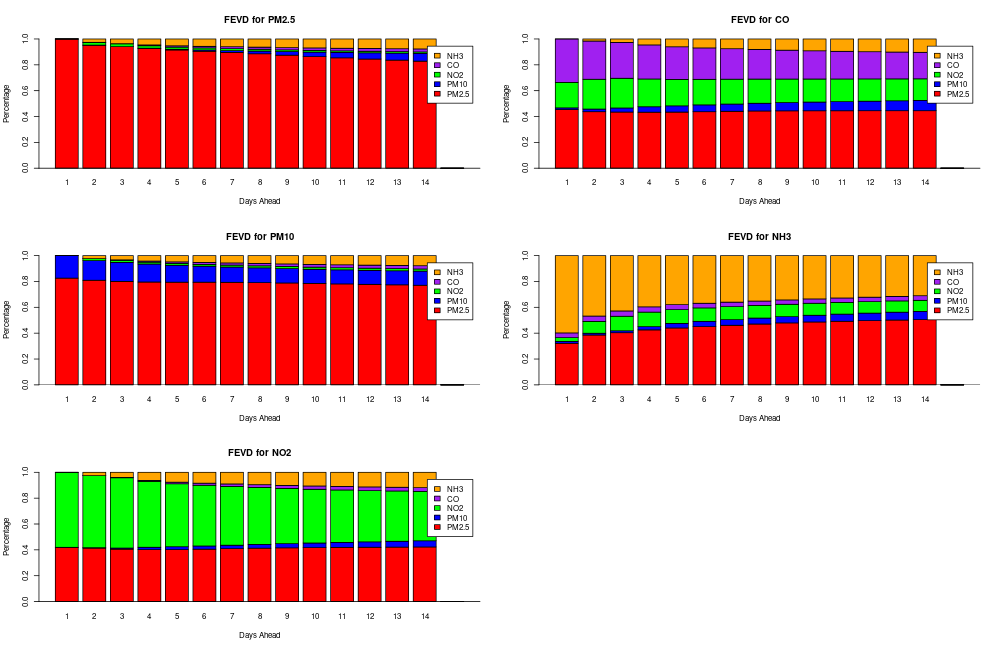
\includegraphics[width=0.9\linewidth]{../analysis/assets/fevd_delhi.png}
        \caption{FEVD of Daily Log1p-Transformed Pollutants (VAR(4) Model, 10-day horizon).}
    \end{figure}
    \begin{itemize}
        \item \footnotesize Large portion of forecast error variance for most pollutants is explained by their own shocks or by $PM_{2.5}$ shocks.
        \item \footnotesize Example: $NO_2$ shocks explain ~17.8\% of $CO$'s forecast error variance at a 10-day horizon.
    \end{itemize}
\end{frame}

%----------------------------------------------------------------------------------------
\begin{frame}
    \frametitle{Forecasting Evaluation: VAR(4) vs. VARMA(1,1)}
    \begin{itemize}
        \item \textbf{Setup:}
            \begin{itemize}
                \item Data split: Training (first 718 days), Test (last 14 days).
                \item Forecast horizon: 14 days ahead.
            \end{itemize}
        \item \textbf{RMSE Comparison on Test Set:}
            \begin{center}
            \footnotesize
            \begin{tabular}{lccccc}
                \toprule
                Model      & $PM_{2.5}$ & $PM_{10}$ & $NO_2$ & $CO$  & $NH_3$ \\
                \midrule
                VAR(4)     & 0.721      & 0.543     & 0.179  & 0.202 & 0.150  \\
                \textbf{VARMA(1,1)} & \textbf{0.605} & \textbf{0.446} & \textbf{0.169} & \textbf{0.189} & \textbf{0.142} \\
                \bottomrule
            \end{tabular}
            \end{center}
            \vspace{0.2cm}
            \textbf{Observation:} VARMA(1,1) showed lower RMSE for all five pollutants, suggesting better forecast accuracy for this dataset and horizon.
    \end{itemize}
\end{frame}

%----------------------------------------------------------------------------------------
\begin{frame}
    \frametitle{Example: VAR(4) Forecasts for Delhi Pollutants}
    \begin{figure}
        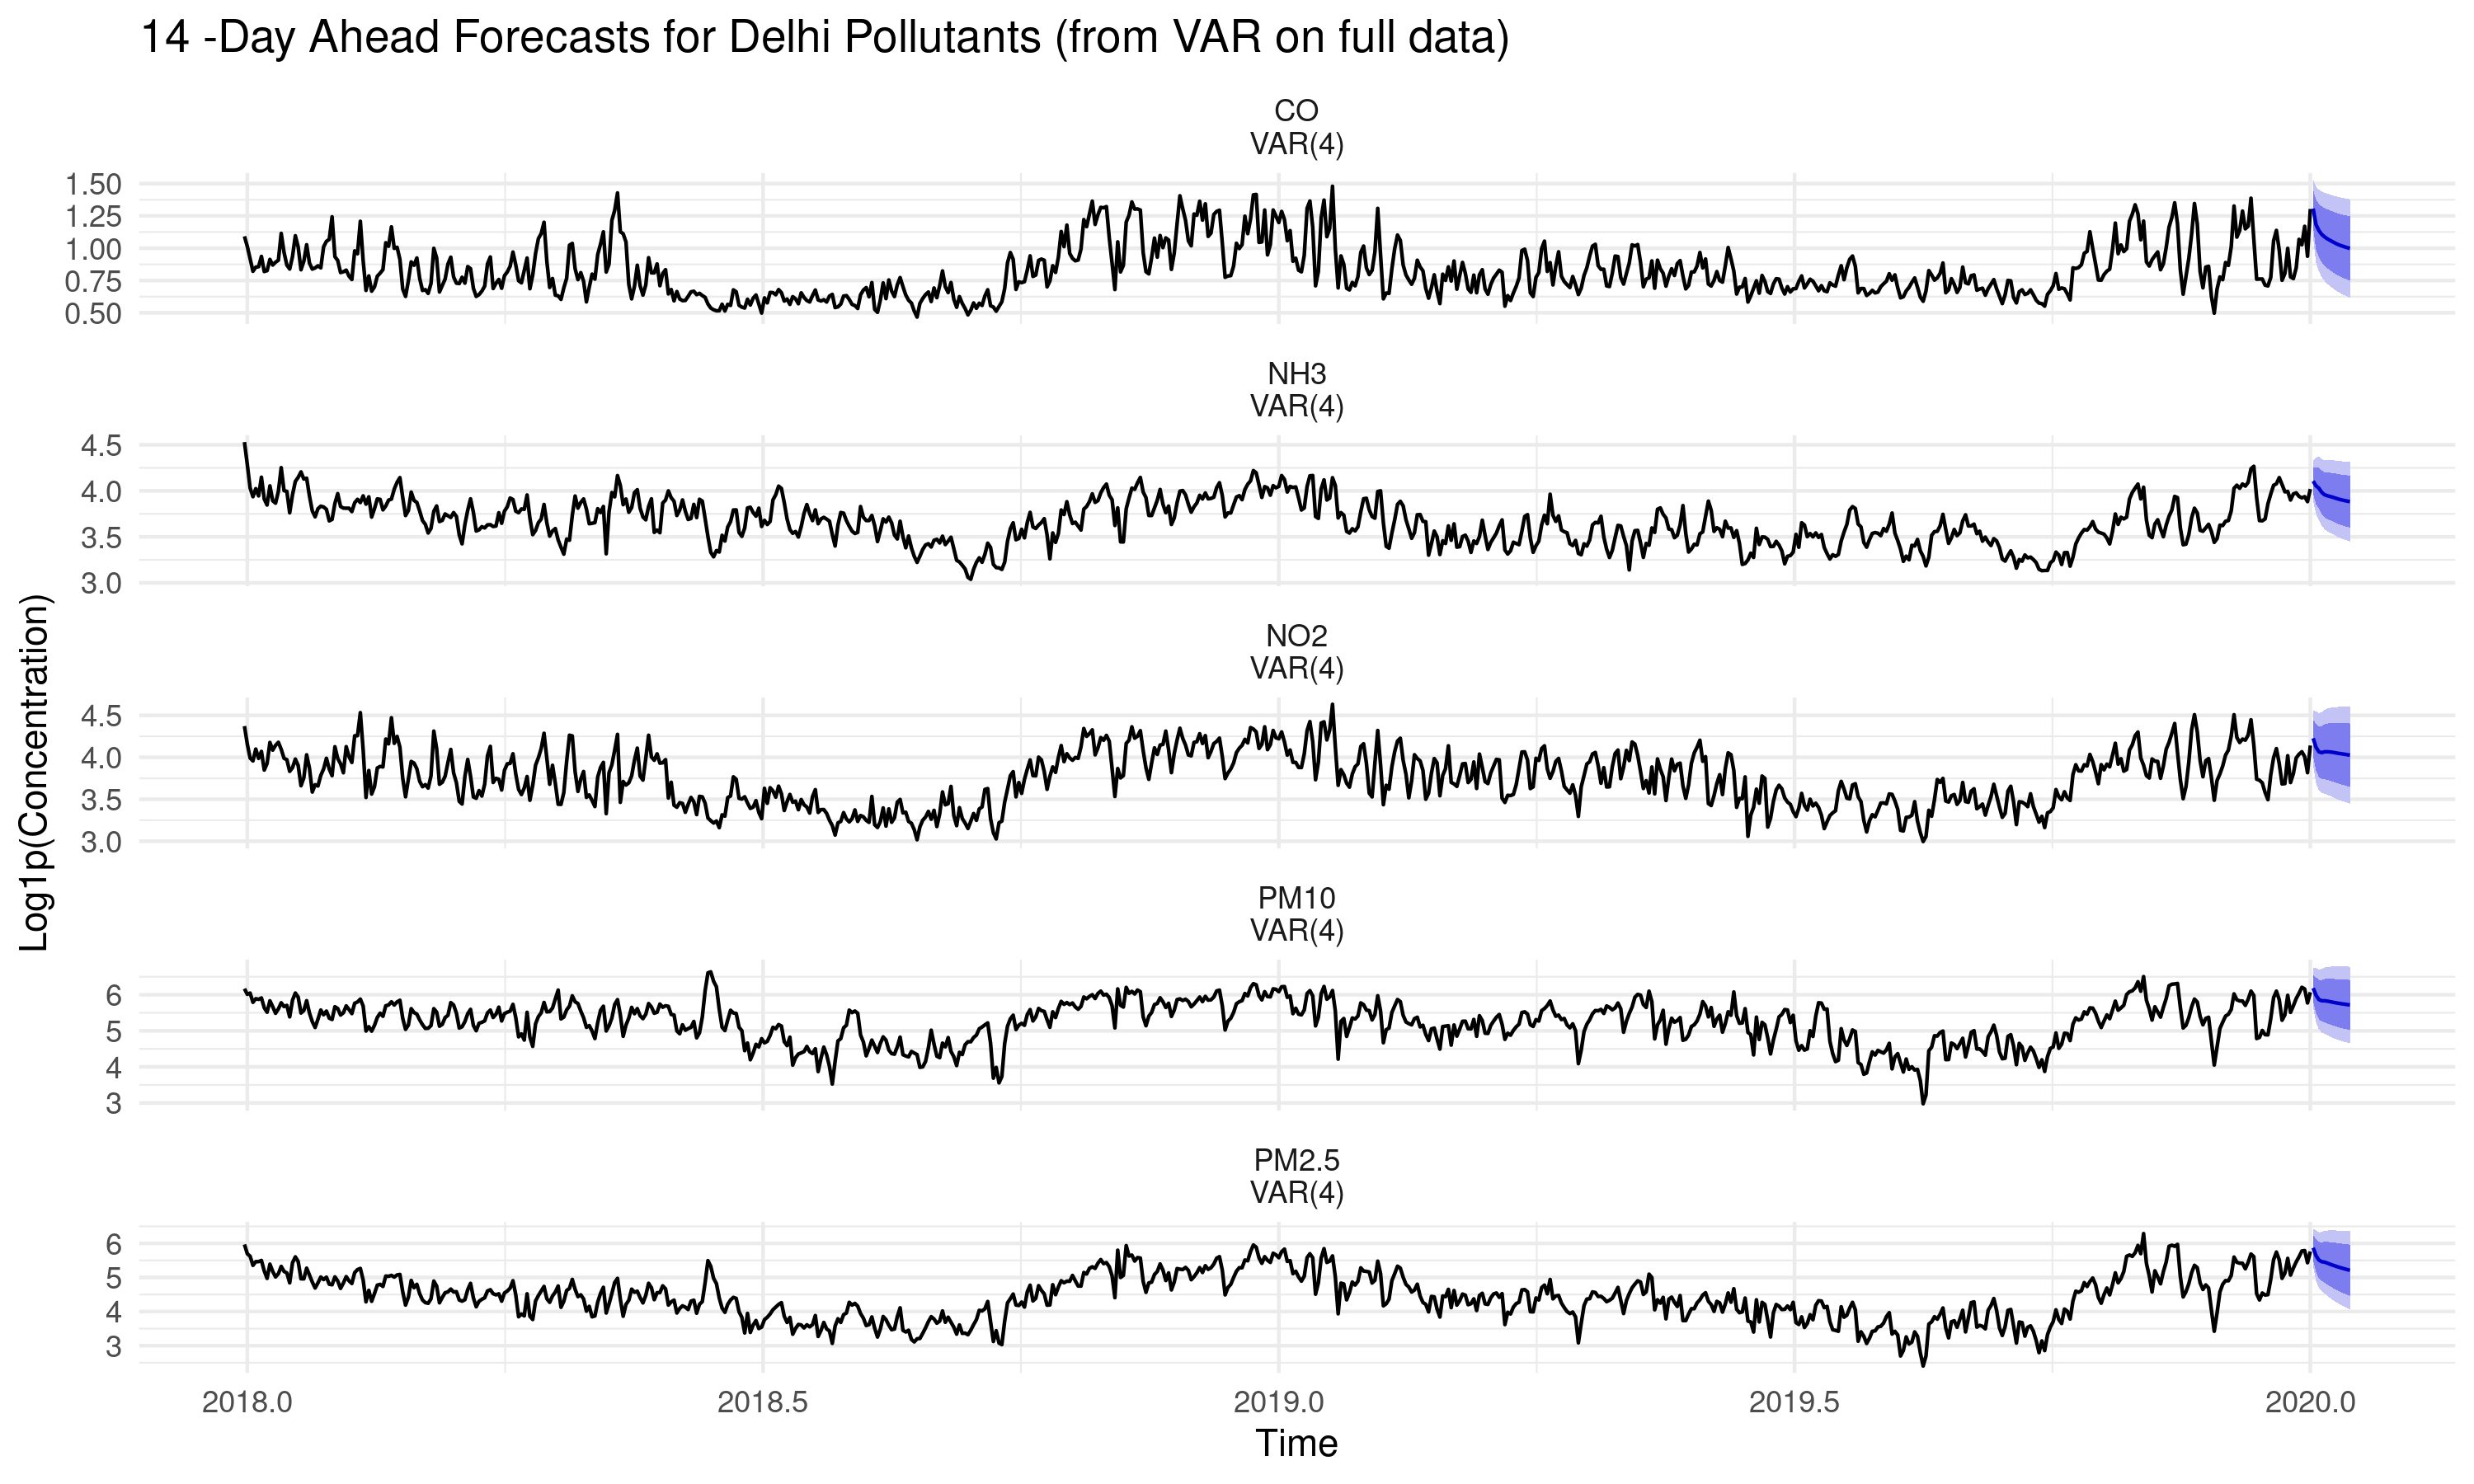
\includegraphics[width=\linewidth]{../analysis/assets/var_forecast_delhi.png}
        \caption{14-Day Ahead Forecasts from VAR(4) Model.}
    \end{figure}
    \begin{itemize}
        \item \footnotesize Forecasts tend to revert to the mean, with widening confidence intervals as the horizon increases.
    \end{itemize}
\end{frame}

%----------------------------------------------------------------------------------------
\section{Conclusion \& Limitations}
%----------------------------------------------------------------------------------------
\begin{frame}
    \frametitle{Conclusion}
    \begin{itemize}
        \item Successfully applied VAR and VARMA models to analyze multivariate dynamics of 5 key air pollutants in Delhi.
        \item Daily log1p-transformed pollutant series were found to be stationary I(0).
        \item VAR(4) model revealed:
            \begin{itemize}
                \item Significant Granger causalities (e.g. $PM_{2.5}$, $NH_3$ influencing others).
                \item Dynamic interactions via IRFs (e.g. $NO_2$ shocks affect other pollutants).
                \item FEVD showed importance of own shocks and $PM_{2.5}$ in forecast error variance.
            \end{itemize}
        \item For 14-day ahead forecasting, VARMA(1,1) outperformed VAR(4) in terms of RMSE.
        \item The study highlights the potential of multivariate time series models for air quality forecasting and understanding pollutant interactions.
    \end{itemize}
\end{frame}

%----------------------------------------------------------------------------------------
\begin{frame}
    \frametitle{Limitations}
    \begin{itemize}
        \item Focus on a single city (Delhi).
        \item Limited set of pollutants.
        \item Daily aggregation might mask hourly dynamics.
        \item VARMA(1,1) order selection was illustrative, not exhaustive.
    \end{itemize}
\end{frame}

%----------------------------------------------------------------------------------------
% Q&A SLIDE
%----------------------------------------------------------------------------------------
\begin{frame}{Thank You!}
	\begin{center}
		\Huge Thank you for your attention!
	\end{center}
\end{frame}

%----------------------------------------------------------------------------------------

\end{document}